\documentclass[10pt]{article}

% small margins
\usepackage[margin=1in]{geometry}

% no large spaces in lists
\usepackage{enumitem}
\setlist{nolistsep}

\usepackage{graphicx}

\title{\vspace{-4em}DCBA 3D Scanning Implementation Concepts}
\author{Troy Astorino \and Turner Bohlen \and Craig Cheney \and Gus Downs}

\begin{document}
\maketitle
\vspace{-4em}
\section{High Level Design Plan}

We are developing a 3D scanner to meet two primary design goals:
\begin{itemize}
\item Low cost -- less than \$500
\item High precision -- 0.25 mm accuracy
\end{itemize}

We are planning on using the structured light technique to perform the 3D
scanning. This involves projecting a known pattern of light onto an object, and
performing triangulation on each identifiable projected point to calculate that
point's position in space. This triangulation is possible because the position
and orientation of both the camera and projector is known.

We believe we will most effective in maintaining low unit costs and high output
accuracy if we perform the scanning inside of a closed box, minimizing ambient
light. The projection system has to be bright enough to overcome ambient light,
and projector cost increases with lumens. Also, ambient light represents noise
in collected images, and that noise would likely be biased, lowering the
accuracy of our inference algorithms.

\begin{figure}[h]
\centering
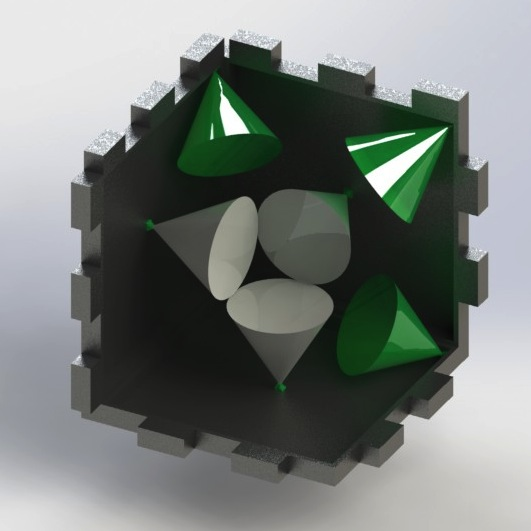
\includegraphics[width=2.5in]{render01.JPG}
\caption{Rough CAD model of overall design concept. The cones represent camera
  fields of view.}
\end{figure}

\section{Projection Concepts}
On the projection side, the resolution of the scan is constrained by the number
of distinguishable lines that are projected onto the object.  This can be achieved by a single projected pattern of sufficient line density (assuming the imaging system can take images to that resolution), or by taking images over multiple projected patterns, where the lines generated by the different patterns hopefully fall on unique parts of the object.

Our concepts for projection are centered about ways to mimic the useful output
of a projector for 3D scanning without incurring the cost of a small digital
projector. We're not entirely sure if that's even necessary, so we also consider
different techniques for integrating a small digital projectors

\begin{itemize}
\item Fine grating in front of an LED. The shadow cast by the grating on the
  object will create the lines necessary for structured light scanning. There are a few different ways this technique can be utilizied. It
  could be achieved by having multiple static LEDs with gratings in front of
  them projecting from different positions.  It could also be achieved with a single LED with a grating in front of it that can be moved by a small piezo-electric motor.
  
  Pros:
  \begin{itemize}
  \item Low cost solution
  \end{itemize}

  Cons:
  \begin{itemize}
  \item Possible issues with diffraction and interference as the grating gets fine enough. (If we had 5 LED sources on a side, want a 4x4 cm grate in front of each LED, implying 75 lines along each dimension of the grating to achieved our desired accuracy.)
  \item Consistency of grating manufacturability with low cost techniques
  \end{itemize}

\item Overlapping color filters. Have multiple filter sheets (red, green, blue, etc.) with holes cut in them. Have the holes overlap irregularly, so a multi-colored grid is projected on the object to be scanned.

Pros:
\begin{itemize}
\item Low cost
\item Avoid interference issues arising from a fine grid with so many slits because light in adjacent grid squares are of different wavelengths.
\end{itemize}

Cons:
\begin{itemize}
\item Projected colored light will be difficult to distinguish on objects that are close in color to the projected light.
\end{itemize}

\item Use an off-the-shelf pico-projector. 

Pros:
\begin{itemize}
\item Reduces number of parts needed in design on our end
\item Aren't stuck with a set projection pattern based on hardware
\end{itemize}

Cons:
\begin{itemize}
\item May not be able to focus at the closest distance we require without changing lenses
\item Cost seems to be around \$350-\$600 per unit
\end{itemize}

\item Manufacture own small projector.

Pros:
\begin{itemize}
\item May allow us to design for a very short focal distance
\item Again, aren't stuck with a set projection pattern based on hardware
\end{itemize}

Cons:
\begin{itemize}
\item Very little idea of what is required for this
\item Adds complexity to design
\item Could also be very expensive
\end{itemize}
\end{itemize}

\section{Imaging Concepts}
On the imaging side, the resolution of the scan is limited by, predictable, the resolution of the camera. The massive use of CMOS arrays in consumer electronics has driven down the cost of high resolution cameras.  Even with a lower resolution camera, however, scan resolution can be increased by taking multiple images, or better, taking images from multiple locations.

Although it may be obvious, it is imperitive that each point in the scan be in focus when the image is taken. For such close up imaging, this can be a challege to gather enough light for the image while retaining a sufficient depth of field. The other challenge is to capture as much of the area inside of the scanner as possible with as few cameras as possible. This would suggest trying to use wide angle cameras, but the cheapest cameras all have a relatively narrow field of view.

\begin{itemize}
\item Array of cheap off-the-shelf CMOS cameras. 

Pros:
\begin{itemize}
\item Can use the cameras that are used in cell phones, allowing us to obtain low-cost high-quality sensors by piggybacking off the volume of these cameras for cell phone manufacturing.
\end{itemize}

Cons:
\begin{itemize}
\item Only in focus for a small range of distances.
\item Small solid angle for field of view
\item Difficulty focusing at small distances from the camera
\end{itemize}

\item Pinhole camera using cheap CMOS arrays.

Pros:
\begin{itemize}
\item Can use the same low cost CMOS arrays as those used in cell phone cameras
\item Objects at any distance are in focus (to the size of the pinhole)
\item Lack of lens could lower cost
\end{itemize}

Cons:
\begin{itemize}
\item Difficult to find off the shelf pinhole cameras, may have to manufacture on our own
\item Issues with collecting enough light
\end{itemize}

\end{itemize}

\end{document}